\section{Ejercicios}

\subsection{Ejercicios de construcción - Pappus}

\begin{section-exercise}
    Aplicar el teorema de Pappus, dada la disposición \hspace{0.3cm}
    \begin{tabular}{|c|c|c|}
        \hline
        A&B&C \\\hline
        F&D&E \\\hline\hline
        && \\\hline
    \end{tabular}
    \vspace*{\fill}
    \begin{figure}[H]
        \centering
        
%dash pattern=on 5pt off 2pt
%[fill = white, rounded corners = 5pt, inner sep=0.8pt]
\begin{tikzpicture}[scale = 1.2]
    \clip(-7.18,-0.99) rectangle (4.94,8.68);
    \draw [line width=1.2pt] (-3.5,4.81) circle (2.98cm);
    \begin{scriptsize}
        \normalsize
        \fill [color=black] (-4.5,7.62) circle (2.5pt);
        \draw[color=black] (-4.75,7.97) node {$A$};
        \fill [color=black] (-2.24,2.11) circle (2.5pt);
        \draw[color=black] (-1.96,1.72) node {$B$};
        \fill [color=black] (-5.84,2.97) circle (2.5pt);
        \draw[color=black] (-6.26,2.86) node {$C$};
        \fill [color=black] (-0.91,3.34) circle (2.5pt);
        \draw[color=black] (-0.54,3.22) node {$D$};
        \fill [color=black] (-0.52,4.85) circle (2.5pt);
        \draw[color=black] (-0.13,5.03) node {$E$};
        \fill [color=black] (-0.72,5.86) circle (2.5pt);
        \draw[color=black] (-0.4,6.13) node {$F$};
    \end{scriptsize}
\end{tikzpicture}
    \end{figure}
    \vspace*{\fill}
\end{section-exercise}

\newpage
\begin{section-exercise}
    Aplicar el teorema de Pappus, dada la disposición \hspace{0.3cm}
    \begin{tabular}{|c|c|c|}
        \hline
        E&D&F \\\hline
        A&C&B \\\hline\hline
        && \\\hline
    \end{tabular}
    \vspace*{\fill}
    \begin{figure}[H]
        \centering
        
%dash pattern=on 5pt off 2pt
%[fill = white, rounded corners = 4pt, inner sep = 1pt]
\begin{tikzpicture}[scale = 1.5]
    \clip(-5.28,-5.51) rectangle (3.8,8.27);
    \draw [line width=1.2pt,domain=-5.28:3.8] plot(\x,{(--8.31-7.4*\x)/-1.15});
    \draw [line width=1.2pt,domain=-5.28:3.8] plot(\x,{(--11.9--3.51*\x)/-0.31});
    \begin{scriptsize}
        \normalsize
        \fill [color=black] (1.98,5.57) circle (2.5pt);
        \draw[color=black] (2.49,5.81) node {$A$};
        \fill [color=black] (0.84,-1.83) circle (2.5pt);
        \draw[color=black] (1.39,-1.79) node {$B$};
        \fill [color=black] (1.42,1.91) circle (2.5pt);
        \draw[color=black] (1.89,1.99) node {$C$};
        \fill [color=black] (-3.6,2.44) circle (2.5pt);
        \draw[color=black] (-4.06,2.39) node {$D$};
        \fill [color=black] (-3.92,5.95) circle (2.5pt);
        \draw[color=black] (-4.39,5.74) node {$E$};
        \fill [color=black] (-3.09,-3.36) circle (2.5pt);
        \draw[color=black] (-3.6,-3.67) node {$F$};
    \end{scriptsize}
\end{tikzpicture}
    \end{figure}
    \vspace*{\fill}
\end{section-exercise}

\newpage
\begin{section-exercise}
    Aplicar el teorema de Pappus, dada la disposición \hspace{0.3cm}
    \begin{tabular}{|c|c|c|}
        \hline
        B&A&C \\\hline
        F&E&D \\\hline\hline
        && \\\hline
    \end{tabular}
    \vspace*{\fill}
    \begin{figure}[H]
        \centering
        
%dash pattern=on 5pt off 2pt
%[fill = white, rounded corners = 5pt, inner sep=0.8pt]
\begin{tikzpicture}[scale = 1.2]
    \clip(-7.87,-1.23) rectangle (2.09,9.26);
    \draw [line width=1.2pt] (-3.5,4.81) circle (3.31cm);
    \begin{scriptsize}
        \normalsize
        \fill [color=black] (-3.5, 4.81) circle (2pt);
        \fill [color=black] (-6.31,6.56) circle (2.5pt);
        \draw[color=black] (-6.62,6.77) node {$D$};
        \fill [color=black] (-1.4,7.36) circle (2.5pt);
        \draw[color=black] (-1.31,7.97) node {$E$};
        \fill [color=black] (-4.48,1.65) circle (2.5pt);
        \draw[color=black] (-4.49,1.15) node {$B$};
        \fill [color=black] (-0.19,4.83) circle (2.5pt);
        \draw[color=black] (0.23,4.95) node {$A$};
        \fill [color=black] (-1.6,2.1) circle (2.5pt);
        \draw[color=black] (-1.51,1.7) node {$C$};
    \end{scriptsize}
\end{tikzpicture}
    \end{figure}
    \vspace*{\fill}
\end{section-exercise}

\newpage
\begin{section-exercise}
    Aplicar el teorema de Pappus, dada la disposición \hspace{0.3cm}
    \begin{tabular}{|c|c|c|}
        \hline
        A&C&B \\\hline
        F&D&E \\\hline\hline
        && \\\hline
    \end{tabular}
    \vspace*{\fill}
    \begin{figure}[H]
        \centering
        
%dash pattern=on 5pt off 2pt
%[fill = white, rounded corners = 5pt, inner sep=0.8pt]
\begin{tikzpicture}[scale = 1.2]
    \clip(-7.14,-1.18) rectangle (6.49,8.66);
    \draw [line width=1.2pt] (2.61,3.83) circle (3.12cm);
    \begin{scriptsize}
        \normalsize
        \fill [color=black] (3.68,6.75) circle (2.5pt);
        \draw[color=black] (3.88,7.23) node {$A$};
        \fill [color=black] (3.93,1) circle (2.5pt);
        \draw[color=black] (4.08,0.55) node {$C$};
        \fill [color=black] (0.75,1.33) circle (2.5pt);
        \draw[color=black] (0.52,0.8) node {$B$};
        \fill [color=black] (5.55,2.78) circle (2.5pt);
        \draw[color=black] (5.92,2.67) node {$D$};
        \fill [color=black] (-0.21,5.16) circle (2.5pt);
        \draw[color=black] (-0.58,5.46) node {$E$};
        \fill [color=black] (-0.49,3.47) circle (2.5pt);
        \draw[color=black] (-0.9,3.22) node {$F$};
    \end{scriptsize}
\end{tikzpicture}
    \end{figure}
    \vspace*{\fill}
\end{section-exercise}

\newpage
\begin{section-exercise}
    Aplicar el teorema de Pappus, dada la disposición \hspace{0.3cm}
    \begin{tabular}{|c|c|c|}
        \hline
        B&F&E \\\hline
        A&C&D \\\hline\hline
        && \\\hline
    \end{tabular}
    \vspace*{\fill}
    \begin{figure}[H]
        \centering
        
%dash pattern=on 5pt off 2pt
%[fill = white, rounded corners = 5pt, inner sep=0.8pt]
\begin{tikzpicture}[scale = 1.8]
    \clip(-5.39,-0.83) rectangle (0.2,9.99);
    \draw [line width=1.2pt] (-3.03,4.71) circle (1.56cm);
    \begin{scriptsize}
        \normalsize
        \fill [color=black] (-3.03,4.71) circle (1.6pt);
        \fill [color=black] (-2.11,3.45) circle (1.8pt);
        \draw[color=black] (-2.09,3.11) node {$A$};
        \fill [color=black] (-1.56,5.21) circle (1.8pt);
        \draw[color=black] (-1.32,5.09) node {$D$};
        \fill [color=black] (-4.32,3.84) circle (1.8pt);
        \draw[color=black] (-4.63,3.57) node {$C$};
        \fill [color=black] (-2.59,6.2) circle (1.8pt);
        \draw[color=black] (-2.54,6.58) node {$B$};
    \end{scriptsize}
\end{tikzpicture}
    \end{figure}
    \vspace*{\fill}
\end{section-exercise}




\newpage
\subsection{Ejercicios de perspectiva - Desargues}

\begin{section-exercise}
    Encuentre, con la ayuda de una regla, el punto y la recta para los cuales los triángulos \theTriangle{ABC} y \theTriangle{XYZ} están en perspectiva.
    \vspace*{\fill}
    \begin{figure}[H]
        \centering
        \definecolor{ttqqcc}{rgb}{0.33,0.33,0.33}
%dash pattern=on 5pt off 2pt
%[fill = white, rounded corners = 4pt, inner sep = 1pt]
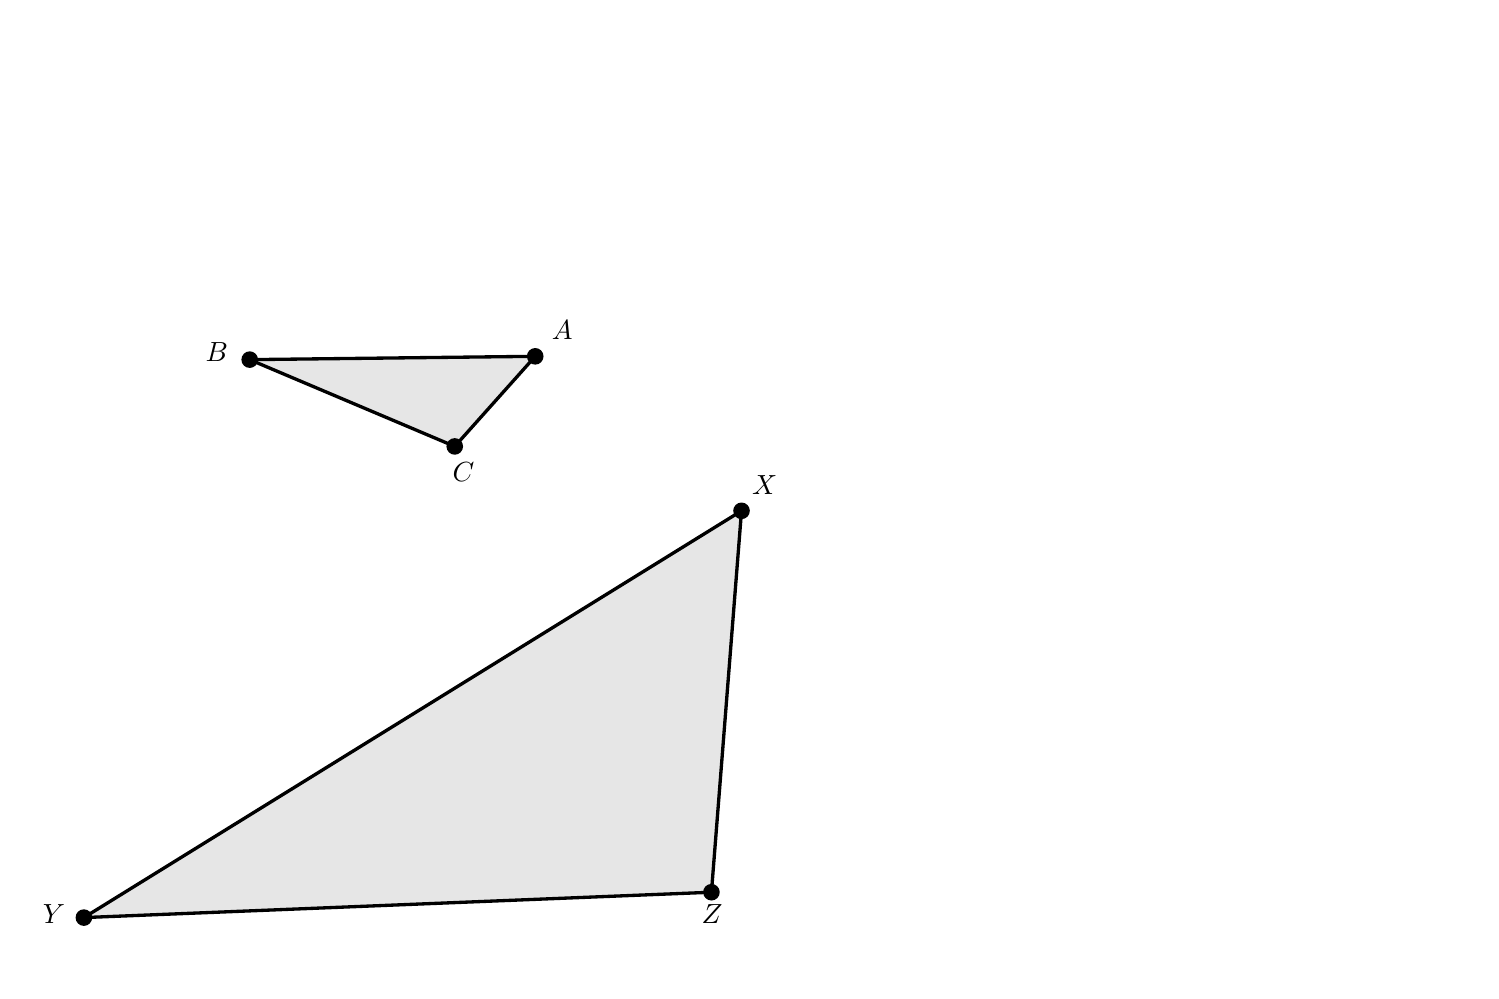
\begin{tikzpicture}[scale = 0.2]
    \clip(-25.62,-26.27) rectangle (66,33.59);
    \fill[line width=0pt,color=ttqqcc,fill=ttqqcc,fill opacity=0.15] (6.61,12.72) -- (-11.52,12.51) -- (1.5,7) -- cycle;
    \fill[line width=0pt,color=ttqqcc,fill=ttqqcc,fill opacity=0.15] (19.71,2.91) -- (-22.05,-22.92) -- (17.8,-21.31) -- cycle;
    \draw [line width=1.2pt] (6.61,12.72)-- (-11.52,12.51);
    \draw [line width=1.2pt] (-11.52,12.51)-- (1.5,7);
    \draw [line width=1.2pt] (1.5,7)-- (6.61,12.72);
    \draw [line width=1.2pt] (19.71,2.91)-- (-22.05,-22.92);
    \draw [line width=1.2pt] (-22.05,-22.92)-- (17.8,-21.31);
    \draw [line width=1.2pt] (17.8,-21.31)-- (19.71,2.91);
    \begin{scriptsize}
        \normalsize
        \fill [color=black] (-11.52,12.51) circle (15pt);
        \draw[color=black] (-13.61,13.01) node {$B$};
        \fill [color=black] (1.5,7) circle (15pt);
        \draw[color=black] (2.06,5.38) node {$C$};
        \fill [color=black] (6.61,12.72) circle (15pt);
        \draw[color=black] (8.33,14.37) node {$A$};
        \fill [color=black] (19.71,2.91) circle (15pt);
        \draw[color=black] (21.18,4.55) node {$X$};
        \fill [color=black] (-22.05,-22.92) circle (15pt);
        \draw[color=black] (-23.95,-22.72) node {$Y$};
        \fill [color=black] (17.8,-21.31) circle (15pt);
        \draw[color=black] (17.84,-22.72) node {$Z$};
    \end{scriptsize}
\end{tikzpicture}
    \end{figure}
    \vspace*{\fill}
\end{section-exercise}

\newpage
\begin{section-exercise}
    Encuentre, con la ayuda de una regla, el punto y la recta para los cuales los triángulos \theTriangle{ABC} y \theTriangle{XYZ} están en perspectiva.
    \vspace*{\fill}
    \begin{figure}[H]
        \centering
        \definecolor{ttqqcc}{rgb}{0.33,0.33,0.33}
%dash pattern=on 5pt off 2pt
%[fill = white, rounded corners = 4pt, inner sep = 1pt]
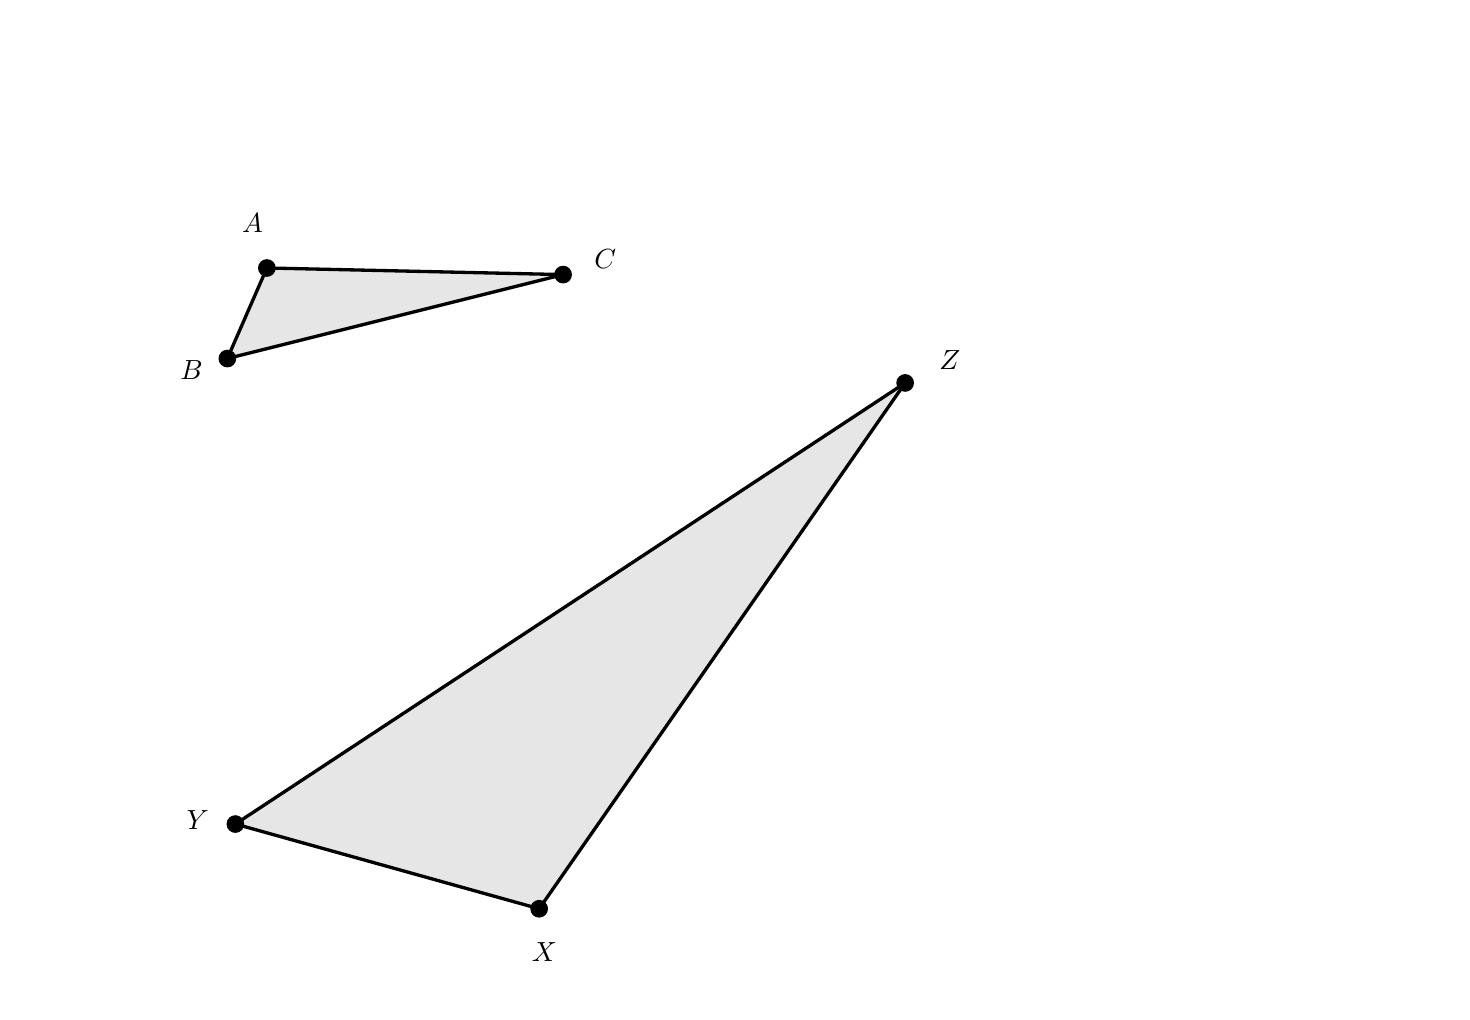
\begin{tikzpicture}[scale = 0.2]
    \clip(-20.65,-28.57) rectangle (69.12,32.66);
    \fill[line width=0pt,color=ttqqcc,fill=ttqqcc,fill opacity=0.15] (-5.46,17.4) -- (-7.97,11.65) -- (13.35,16.98) -- cycle;
    \fill[line width=0pt,color=ttqqcc,fill=ttqqcc,fill opacity=0.15] (11.83,-23.29) -- (-7.46,-17.91) -- (35.07,10.1) -- cycle;
    \draw [line width=1.2pt] (-5.46,17.4)-- (-7.97,11.65);
    \draw [line width=1.2pt] (-7.97,11.65)-- (13.35,16.98);
    \draw [line width=1.2pt] (13.35,16.98)-- (-5.46,17.4);
    \draw [line width=1.2pt] (11.83,-23.29)-- (-7.46,-17.91);
    \draw [line width=1.2pt] (-7.46,-17.91)-- (35.07,10.1);
    \draw [line width=1.2pt] (35.07,10.1)-- (11.83,-23.29);
    \begin{scriptsize}
        \normalsize
        \fill [color=black] (-7.97,11.65) circle (16pt);
        \draw[color=black] (-10.25,10.92) node {$B$};
        \fill [color=black] (13.35,16.98) circle (16pt);
        \draw[color=black] (16.03,17.99) node {$C$};
        \fill [color=black] (-5.46,17.4) circle (16pt);
        \draw[color=black] (-6.38,20.25) node {$A$};
        \fill [color=black] (11.83,-23.29) circle (16pt);
        \draw[color=black] (12.16,-26.03) node {$X$};
        \fill [color=black] (-7.46,-17.91) circle (16pt);
        \draw[color=black] (-9.85,-17.63) node {$Y$};
        \fill [color=black] (35.07,10.1) circle (16pt);
        \draw[color=black] (37.91,11.58) node {$Z$};
    \end{scriptsize}
\end{tikzpicture}
    \end{figure}
    \vspace*{\fill}
\end{section-exercise}

\newpage
\begin{section-exercise}
    Encuentre, con la ayuda de una regla, el punto y la recta para los cuales los triángulos \theTriangle{SET} y \theTriangle{DHR} están en perspectiva.
    \vspace*{\fill}
    \begin{figure}[H]
        \centering
        \definecolor{ttqqcc}{rgb}{0.33,0.33,0.33}
%dash pattern=on 5pt off 2pt
%[fill = white, rounded corners = 4pt, inner sep = 1pt]
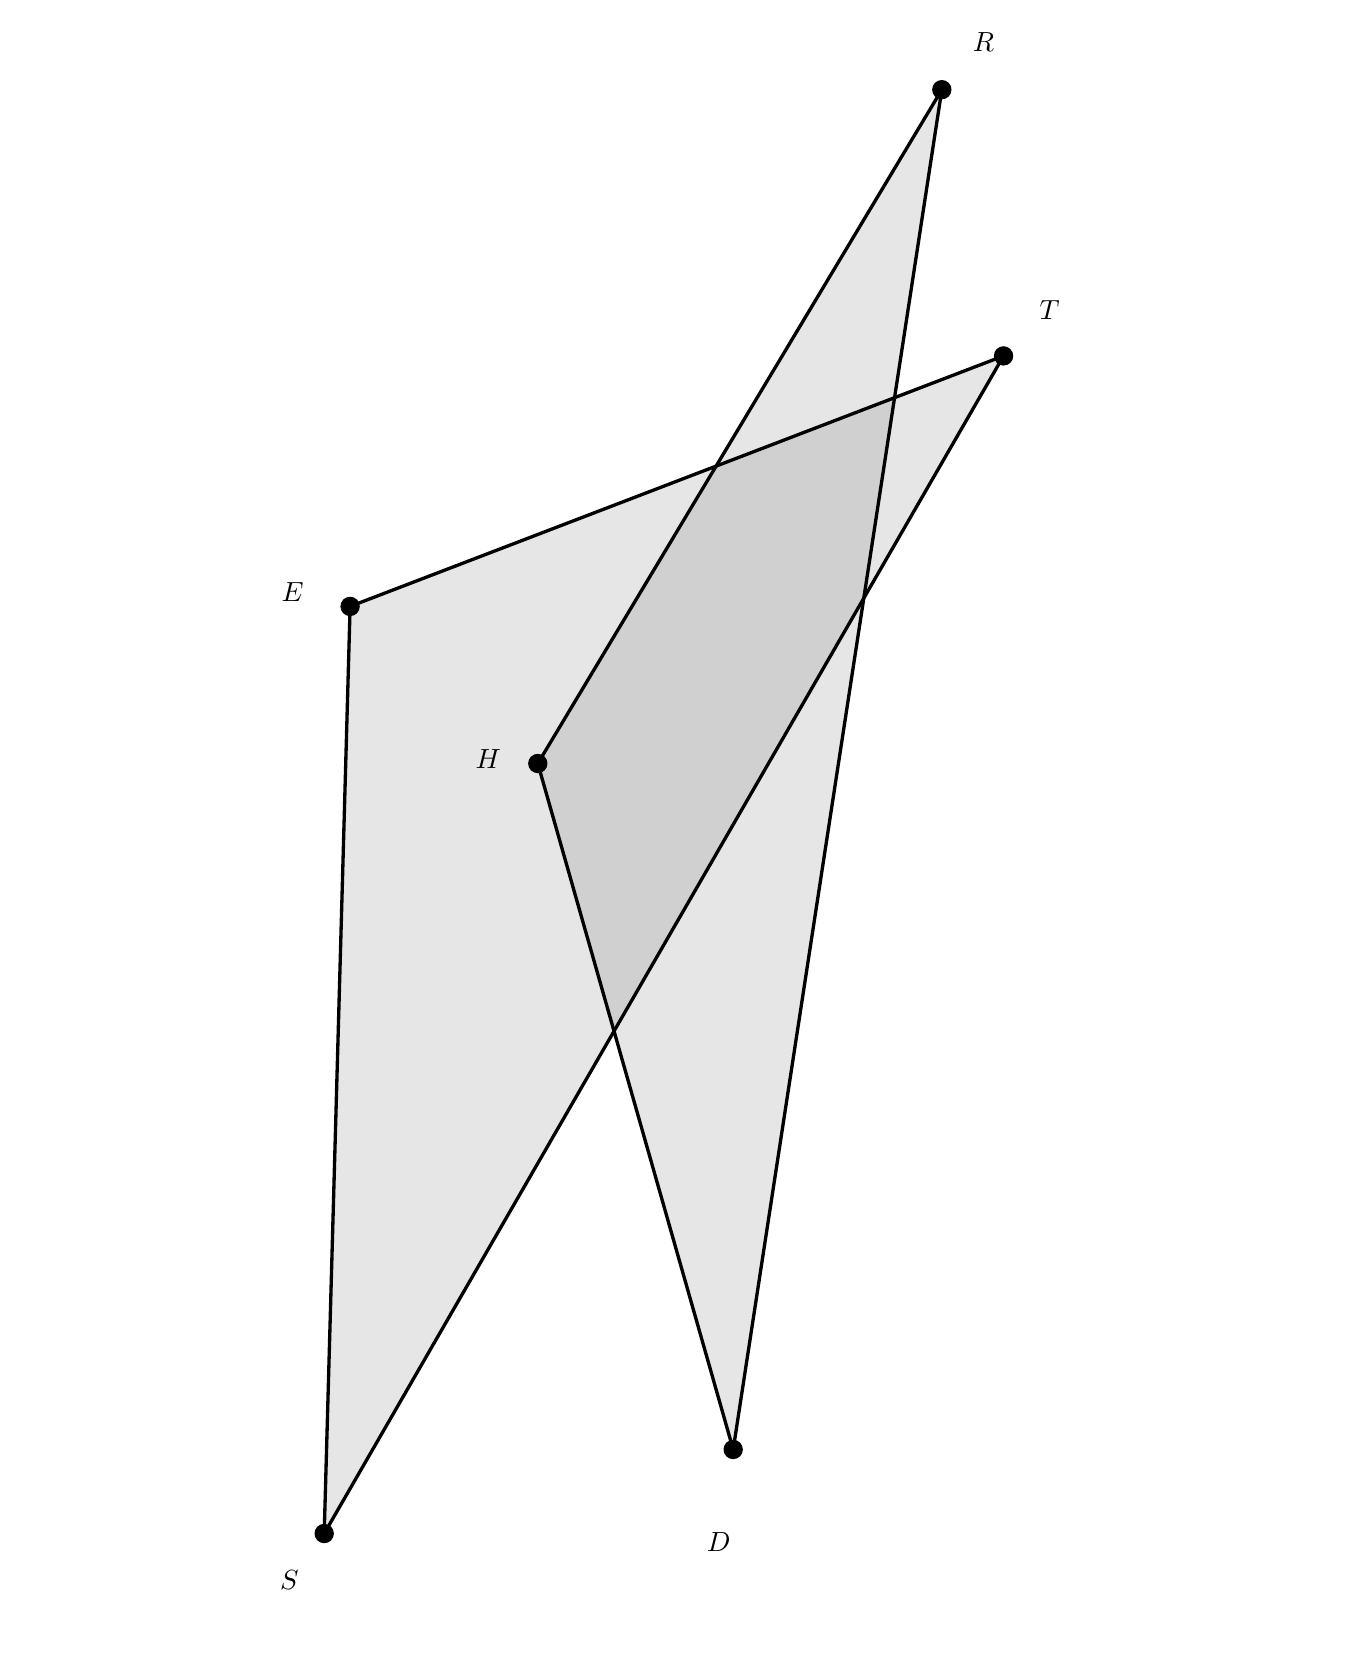
\begin{tikzpicture}[scale = 0.35]
    \clip(-25.62,-26.69) rectangle (21.49,31.61);
    \fill[line width=0pt,color=ttqqcc,fill=ttqqcc,fill opacity=0.15] (9.79,19.7) -- (-13.92,10.61) -- (-14.86,-23.03) -- cycle;
    \fill[line width=0pt,color=ttqqcc,fill=ttqqcc,fill opacity=0.15] (7.55,29.36) -- (-7.11,4.91) -- (-0.02,-19.98) -- cycle;
    \draw [line width=1.2pt] (9.79,19.7)-- (-13.92,10.61);
    \draw [line width=1.2pt] (-13.92,10.61)-- (-14.86,-23.03);
    \draw [line width=1.2pt] (-14.86,-23.03)-- (9.79,19.7);
    \draw [line width=1.2pt] (7.55,29.36)-- (-7.11,4.91);
    \draw [line width=1.2pt] (-7.11,4.91)-- (-0.02,-19.98);
    \draw [line width=1.2pt] (-0.02,-19.98)-- (7.55,29.36);
    \begin{scriptsize}
        \normalsize
        \fill [color=black] (-13.92,10.61) circle (10pt);
        \draw[color=black] (-16.01,11.13) node {$E$};
        \fill [color=black] (-14.86,-23.03) circle (10pt);
        \draw[color=black] (-16.12,-24.7) node {$S$};
        \fill [color=black] (9.79,19.7) circle (10pt);
        \draw[color=black] (11.46,21.37) node {$T$};
        \fill [color=black] (7.55,29.36) circle (10pt);
        \draw[color=black] (9.06,31.08) node {$R$};
        \fill [color=black] (-7.11,4.91) circle (10pt);
        \draw[color=black] (-8.91,5.07) node {$H$};
        \fill [color=black] (-0.02,-19.98) circle (10pt);
        \draw[color=black] (-0.55,-23.35) node {$D$};
    \end{scriptsize}
\end{tikzpicture}
    \end{figure}
    \vspace*{\fill}
\end{section-exercise}

\newpage
\begin{section-exercise}
    Encuentre, con la ayuda de una regla, el punto y la recta para los cuales los triángulos \theTriangle{DEF} y \theTriangle{ABC} están en perspectiva.
    \vspace*{\fill}
    \begin{figure}[H]
        \centering
        \definecolor{ttqqff}{rgb}{0.33,0.33,0.33}
%dash pattern=on 5pt off 2pt
%[fill = white, rounded corners = 4pt, inner sep = 1pt]
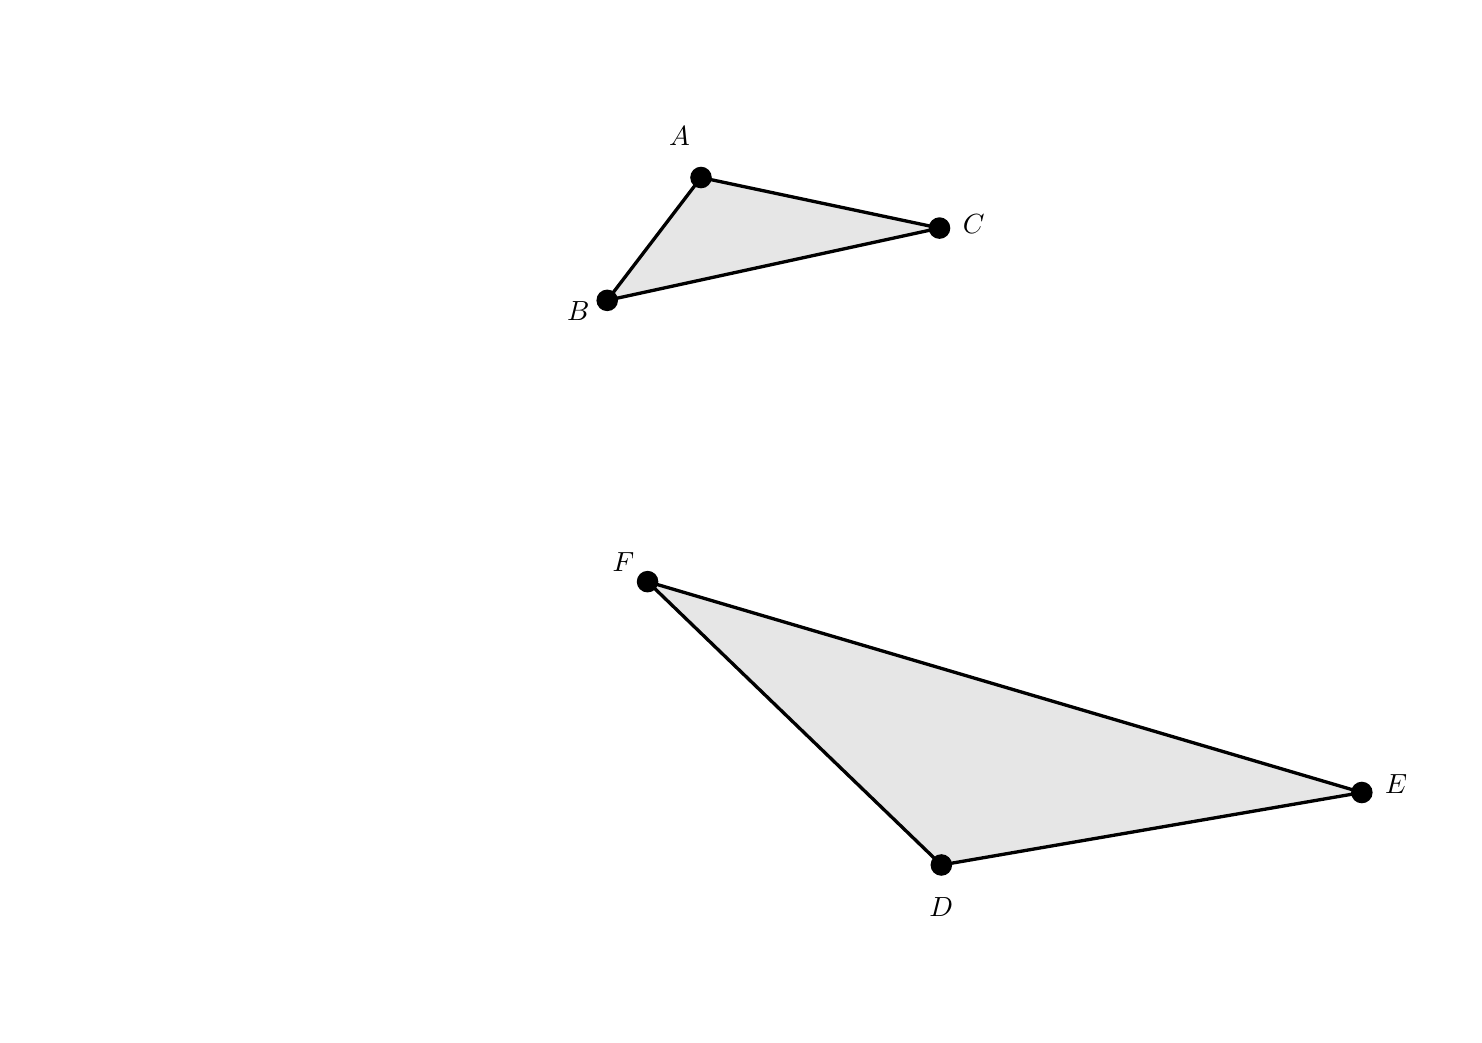
\begin{tikzpicture}[scale = 0.26]
    \clip(-26.68,-15.89) rectangle (42.99,32.35);
    \fill[line width=0pt,color=ttqqff,fill=ttqqff,fill opacity=0.15] (6.21,25.03) -- (1.63,19.03) -- (17.86,22.56) -- cycle;
    \fill[line width=0pt,color=ttqqff,fill=ttqqff,fill opacity=0.15] (17.95,-8.55) -- (38.49,-5.01) -- (3.6,5.29) -- cycle;
    \draw [line width=1.2pt] (6.21,25.03)-- (1.63,19.03);
    \draw [line width=1.2pt] (1.63,19.03)-- (17.86,22.56);
    \draw [line width=1.2pt] (17.86,22.56)-- (6.21,25.03);
    \draw [line width=1.2pt] (17.95,-8.55)-- (38.49,-5.01);
    \draw [line width=1.2pt] (38.49,-5.01)-- (3.6,5.29);
    \draw [line width=1.2pt] (3.6,5.29)-- (17.95,-8.55);
    \begin{scriptsize}
        \normalsize
        \fill [color=black] (1.63,19.03) circle (15pt);
        \draw[color=black] (0.22,18.5) node {$B$};
        \fill [color=black] (17.86,22.56) circle (15pt);
        \draw[color=black] (19.53,22.74) node {$C$};
        \fill [color=black] (6.21,25.03) circle (15pt);
        \draw[color=black] (5.16,27.06) node {$A$};
        \fill [color=black] (17.95,-8.55) circle (15pt);
        \draw[color=black] (17.94,-10.6) node {$D$};
        \fill [color=black] (38.49,-5.01) circle (15pt);
        \draw[color=black] (40.17,-4.6) node {$E$};
        \fill [color=black] (3.6,5.29) circle (15pt);
        \draw[color=black] (2.42,6.24) node {$F$};
    \end{scriptsize}
\end{tikzpicture}
    \end{figure}
    \vspace*{\fill}
\end{section-exercise}

\newpage
\begin{section-exercise}
    Encuentre, con la ayuda de una regla, el punto y la recta para los cuales los triángulos \theTriangle{FED} y \theTriangle{XYZ} están en perspectiva.
    \vspace*{\fill}
    \begin{figure}[H]
        \centering
        
%dash pattern=on 5pt off 2pt
%[fill = white, rounded corners = 5pt, inner sep=0.8pt]
\begin{tikzpicture}[scale = 1.4]
    \clip(-4.83,-8.38) rectangle (5.16,5.19);
    \draw [line width=1.2pt] (0.35,1.15) circle (2.64cm);
    \begin{scriptsize}
        \normalsize
        \fill [color=black] (-2.04,3.44) circle (2.0pt);
        \draw[color=black] (-2.16,3.92) node {$E$};
        \fill [color=black] (-3.33,-7.78) circle (2.0pt);
        \draw[color=black] (-3.64,-7.98) node {$B$};
        \fill [color=black] (2.43,-0.47) circle (2.0pt);
        \draw[color=black] (2.84,-0.64) node {$F$};
        \fill [color=black] (4.03,1.61) circle (2.0pt);
        \draw[color=black] (4.39,1.39) node {$D$};
        \fill [color=black] (1.99,3.22) circle (2.0pt);
        \draw[color=black] (2.19,3.59) node {$A$};
        \fill [color=black] (1.09,3.95) circle (2.0pt);
        \draw[color=black] (1.26,4.31) node {$C$};
    \end{scriptsize}
\end{tikzpicture}
    \end{figure}
    \vspace*{\fill}
\end{section-exercise}